%\documentclass{standalone}
%\usepackage{tikz}

\usetikzlibrary{shapes,arrows,fit,calc,positioning,snakes}
\tikzstyle{input} = [coordinate]
\tikzstyle{output} = [coordinate]
\tikzstyle{box} = [draw, rectangle, fill=white, rounded corners, thick, text width=7em, text centered, minimum height=5em, node distance=3cm]
\tikzstyle{romb} = [draw, diamond, fill=white, thick, text width=5em, text centered, minimum height=5em]
\tikzstyle{container} = [draw, rectangle, dashed, inner sep=1em, node distance=5em]
\tikzstyle{line} = [draw, thick, -latex']
%\begin{document}
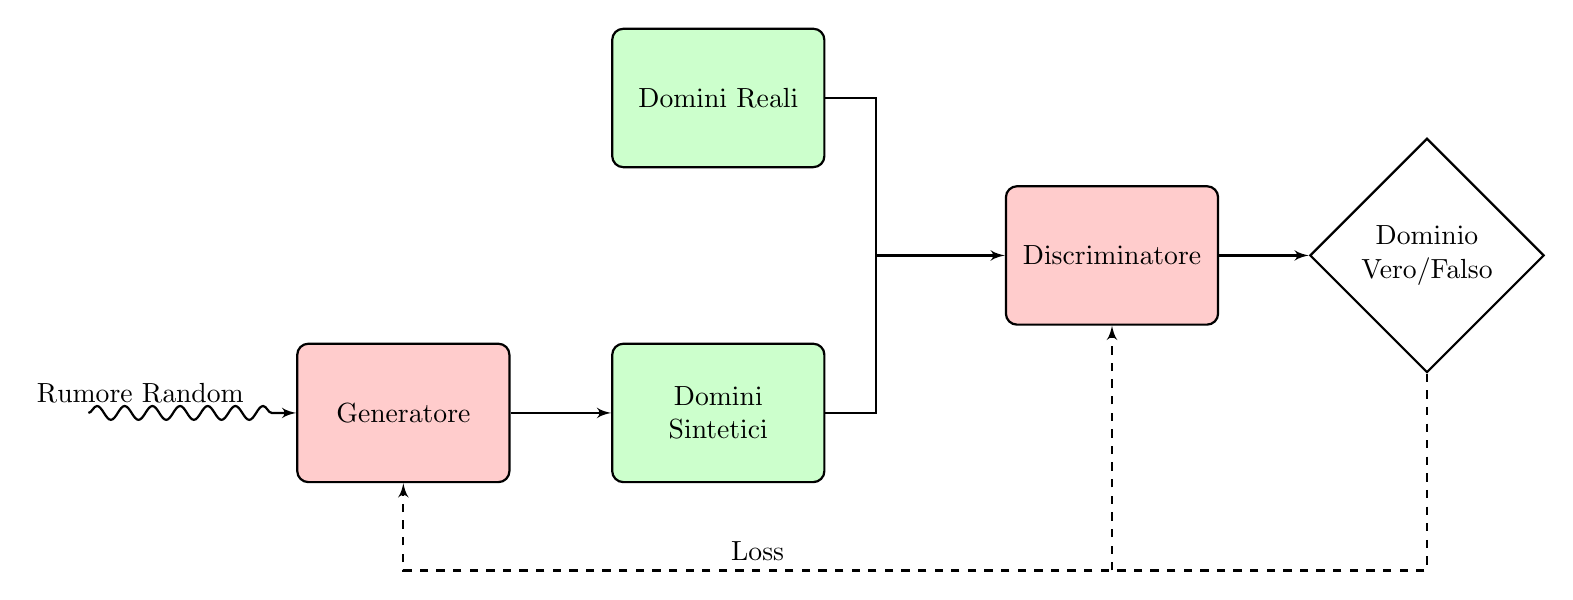
\begin{tikzpicture}[auto, node distance=4cm]
	\coordinate (inters){};
	\node[box, right of=inters,fill=red!20](disc){Discriminatore};
	\node[box, above of=inters,left of=inters, node distance=2cm and 3cm,fill=green!20](dts){Domini Reali};
	\node[box, below of=inters,left of=inters, node distance=2cm and 3cm,fill=green!20](fak){Domini Sintetici};
	\node[box, left of=fak, node distance=4cm,fill=red!20](gen){Generatore};
	\node[input, left of=gen](noise){};
	\node[romb, right of=disc](dec){Dominio Vero/Falso};	
	\coordinate[below of=disc,node distance=4cm](aux){};	
	
	\draw [line,snake=snake,line after snake=2mm](noise) -- node[near start]{Rumore Random}(gen);
	\path [line](disc) -- (dec);
	\path [line] (gen)--(fak);
	\draw [thick] (dts) -| (inters);
	\draw [thick] (fak) -| (inters);
	\path [line] (inters) -- (disc);
	\draw [thick, dashed, -latex'] (dec) |- (aux) -| node[above, near start]{Loss}(gen);
	\draw [thick, dashed, -latex'] (aux) -- (disc);
\end{tikzpicture}
%\end{document}